\documentclass[12pt,twoside]{article}

% packages
\usepackage{amssymb,amsmath,amsbsy}
\usepackage{graphicx}
\usepackage[includeheadfoot, top=1in, bottom=1in, hmargin=1in]{geometry}
\usepackage{fancyhdr}
\usepackage{verbatim}
\usepackage{url}
\usepackage{enumitem}
\usepackage{multicol}

% commands
\newcommand{\given}{\,|\,}
\newcommand{\dd}{\mathrm{d}}
\newcommand{\msun}{\mathrm{M}_\odot}
\newcommand{\projectname}[1]{\begin{center} {\huge {#1}} \end{center}}
\newcommand{\kms}{$\mathrm{km}~\mathrm{s}^{-1}$}

% environments
\newcommand{\problemname}{Problem}
\newcounter{problem}
\newenvironment{problem}{\paragraph{\problemname~\theproblem:}\refstepcounter{problem}}{}
\newenvironment{problem0}{\paragraph{\problemname~0:}}{}
 
\pagestyle{fancy}

\lhead{Project 1}
\chead{}
\rhead{Adrian Price-Whelan}
\lfoot{Galactic Dynamics}
\cfoot{\thepage}
\rfoot{Fall 2014}

\begin{document}

\projectname{The Milky Way}

\begin{problem0}
To get started, 
	\begin{enumerate}
		\item install \texttt{Python} using the \texttt{Anaconda}\footnote{\url{https://store.continuum.io/cshop/anaconda}} distribution;
		\item update \texttt{Conda} and other packages by running:
			\begin{verbatim}
    % conda update conda
    % conda update numpy scipy astropy ipython
			\end{verbatim}
		\item install the package \texttt{Emcee} using \texttt{Conda}:
			\begin{verbatim}
    % conda install emcee
			\end{verbatim}
		\item verify that your installation worked by starting \texttt{IPython} and importing these packages:
			\begin{verbatim}
    % ipython
    In [1]: import numpy
    In [2]: import scipy.optimize
    In [3]: import astropy.coordinates
			\end{verbatim}
			you should not see any errors;
		\item download the tarball for this project which contains the Hipparcos data (as a text file) and some example code.\footnote{Link to data will come via email...}
		
	\end{enumerate}
	
The data file contains kinematic information for $\sim$120,000 stars observed during the Hipparcos astrometric mission. The columns in the data file are:
\begin{multicols}{2}
	\begin{enumerate}[align=left,leftmargin=!,label={\bf Col. \arabic*:}]
		\item Hipparcos ID
		\item Galactic longitude, $l$ (degree)
		\item Galactic latitude, $b$ (degree)
		\item Parallax, $\pi$ (mas)
		\item Proper motion in $l$, $\mu_l$ (mas~yr$^{-1}$)
		\item Proper motion in $b$, $\mu_b$ (mas~yr$^{-1}$)
		\item Uncertainty in $\pi$, $\sigma_\pi$ (mas)
		\item Uncertainty in $\mu_l$, $\sigma_{\mu_l}$ (mas)
		\item Uncertainty in $\mu_b$, $\sigma_{\mu_b}$ (mas)
		\item $V$ magnitude
		\item $B-V$ color
		\item Multiplicity flag (you want this to be 0)
	\end{enumerate}
\end{multicols}
\end{problem0}

\begin{problem} 
The goal is to read in the data file and generate a Hertzsprung-Russell diagram from the data. You'll need to use the parallax to get a distance to each star, then convert the apparent $V$-band magnitude into an absolute magnitude. You will want to select a sub-sample of stars that have good parallax measurements (e.g., $\sigma_\pi / \pi \lesssim 10\%$ or whatever you want) so that the distance conversions make sense. Even with this cut, you might end up with some strange outliers -- check that there are no crazy distance outliers.

You will also want to remove binary and multiple star systems from your sample. Do this by requiring that the multiplicity field is 0.

Make a plot of the $B-V$ color vs. absolute $V$-band magnitude for all stars remaining in your sample. Set the $x$-axis limits to $(-0.5,2.)$ and the $y$-axis limits to $(15,-5)$ -- note the inversion. Do you notice anything strange about the distribution of points in this plot? Extra credit if you make a \emph{density} plot instead of a scatter plot by making a 2D histogram of the data (e.g., right panel of figure below).

\begin{figure}[!h]
\begin{center}
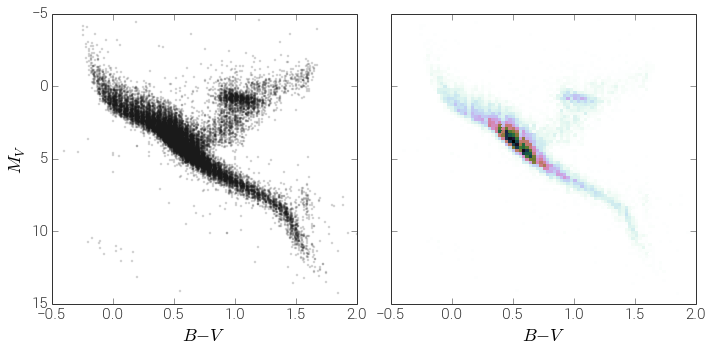
\includegraphics[width=\textwidth]{hr-diag.png}
\caption{ H-R diagram of Hipparcos stars. }\label{fig:hrdiag}
\end{center}
\end{figure}

\end{problem}

\begin{problem}
Now we will try to estimate the Oort constants ($A$,$B$) from the Hipparcos proper motions. 

\noindent{\bf a)} First derive the Oort constants ($A$, $B$) in terms of the rotation curve, $v_c(R)$. What assumptions do you have to make along the way? Are these assumptions more likely to be valid for stars or gas? What is the physical interpretation of the Oort constants?

\bigskip
\noindent{\bf b)} Now derive a relation between the proper motion in Galactic longitude (or tangential velocity), distance, and Galactic longitude in terms of the Oort constants. 

%Assuming the rotation curve of the Milky Way near the solar neighborhood is flat and that stars (and the Sun) are on circular orbits in the Galactic midplane, the transverse velocity, $v_{\rm t}$, of a star at distance $d$ and Galactic longitude $l$ can be found from the relation
%\begin{equation}
%	v_{\rm t} = Ad\cos(2l) + Bd
%\end{equation}
%(this also assumes that the Galactic potential is axisymmetric). Keeping in mind the strong assumptions made above, we can divide both sides by the distance and derive a relation to predict the proper motion of a star given its Galactic longitude:
%\begin{equation}
%	v_{\rm t}/d = \mu_l = A\cos(2l) + B.
%\end{equation}
%The Oort constants are typically expressed in units of $\mathrm{km}/\mathrm{s}/\mathrm{kpc}$, but proper motions are typically given in $\mathrm{mas}/\mathrm{yr}$. To convert a proper motion from one to the other we just have to divide by a conversion factor:
%\begin{equation}
%	\mu_l = \frac{A\cos(2l) + B}{4.7405}
%\end{equation}
%where $\mu_l$ is now $\mathrm{mas}/\mathrm{yr}$ and $A$ and $B$ are in $\mathrm{km}/\mathrm{s}/\mathrm{kpc}$. 
\bigskip
\noindent{\bf c)} The Hipparcos data contains positions and proper motions ($l$ and $\mu_l$) for a large sample of stars in the solar neighborhood. We can therefore use these data to infer values of the Oort constants using the relation above. The uncertainties in the proper motions are much larger than the uncertainties in the longitude (measuring position on the sky is much easier than measuring a proper motion), so this problem is analogous to the classic problem of fitting a line to data where the ``$y$'' data are the proper motions, the ``$x$'' data are the (cosine of the) Galactic longitudes, and we can neglect the uncertainties on $x$.\footnote{See \url{http://arxiv.org/abs/1008.4686} for a review on this problem.}
\begin{align}
	x &\iff \cos{2l} \\
	y &\iff \mu_l \\
	\sigma_y &\iff \sigma_{\mu_l}
\end{align}

If we assume that the uncertainties in the proper motions are Gaussian, we can construct a generative model for the observed data as follows: we assume that the observed proper motions can be derived exactly from a line, but that each data point deviates from this perfect straight line because (1) stars have an isotropic random velocity with magnitude drawn from a Gaussian with variance $\sigma_v^2$, and (2) each ``true'' value gets further scattered by a small offset (due to observational uncertainties) drawn from a Gaussian distribution of zero mean and known variance, $\sigma^2_{\mu_l}$. In this model, given an independent Galactic longitude, $l_i$, uncertainty $\sigma_{\mu_l, i}$, Oort constants $A$ and $B$, and velocity dispersion, $\sigma_v$, the probability density $p(\mu_{l,i} \given l_i, \sigma_{\mu_l,i}, A, B)$ of the proper motion, $\mu_{l,i}$, is
\begin{equation}
	p(\mu_{l,i} \given l_i, \sigma^2_{\mu_l,i}, A, B, \sigma_v^2) = \frac{1}{\sqrt{2\pi (\sigma_{\mu_l,i}^2 + \sigma_v^2)}}\exp \left( - \frac{[\mu_{l,i} - {\rm model}(l_i,A,B)]^2}{2[\sigma_{\mu_l,i}^2 + \sigma_v^2]}\right)\label{eq:conditional}
\end{equation}

We then seek the line (Oort constants $A$, $B$) that maximizes the probability of the observed data given the model: the \emph{likelihood}. We assume that the measurements for each star (the data points) are independently drawn so that the total likelihood over $N$ stars is simply the product of the conditional probabilities for each star (Equation~\ref{eq:conditional}):
\begin{equation}
	\mathcal{L} = \prod^N_i p(\mu_{l,i} \given l_i, \sigma^2_{\mu_l,i}, A, B, \sigma_v^2)
\end{equation}

It is often more tractable to deal with the logarithm of the likelihood:
\begin{equation}
	\ln \mathcal{L} = -\frac{1}{2}\ln(2\pi[\sigma_{\mu_l,i}^2 + \sigma_v^2]) - \sum^N_i \frac{[\mu_{l,i} - {\rm model}(l_i,A,B)]^2}{2[\sigma_{\mu_l,i}^2 + \sigma_v^2]}\label{eq:lnlike}
\end{equation}

For this exercise, we will fix the isotropic velocity dispersion to 25~\kms (how bad is this assumption?). If we fix this dispersion, the first factor on the RHS of Equation~\ref{eq:lnlike} is a constant (let's call it $K$). The second term on the RHS is simply $\chi^2$.
\begin{equation}
	\ln \mathcal{L} = K - \frac{1}{2}\chi^2
\end{equation}

You now have two choices. You can either treat this as a $\chi^2$ and plug this in to a least squares optimization routine (e.g., in \texttt{Python}: \texttt{scipy.optimize.leastsq}). Or, you can go Bayesian and turn this into a posterior probability by defining priors on your model parameters, then use an MCMC algorithm (e.g., in \texttt{Python}: \texttt{emcee}) to sample from your posterior distribution. The advantage of the latter approach is that you can easily derive uncertainties over the inferred Oort constants and it requires only a minimal amount of more work.\footnote{Example code that demonstrates using both methods to fit a line to generated data is included in the tarball you downloaded}

What values did you find for the Oort constants, and what uncertainties? How do these (both values and uncertainties) compare to those derived from the Hipparcos team:
\begin{align}
	A &= 14.82 \pm 0.84~\mathrm{km}~\mathrm{s}^{-1}~\mathrm{kpc}^{-1}\\
	B &= -12.37 \pm 0.64~\mathrm{km}~\mathrm{s}^{-1}~\mathrm{kpc}^{-1}
\end{align}

Repeat the above procedure for finding the Oort constants by selecting only Main Sequence stars (use the HR diagram from Problem 1). What values do you get now? 

\pagebreak
\noindent{\bf Extra credit:} A better model for the proper motion data would include the isotropic velocity dispersion as a model parameter. This means not treating the first term on the RHS of Equation~\ref{eq:lnlike} as a constant, and adding a prior for the extra variance. An even better model would also account for the fact that some fraction of the stars will be genuine outliers. We could add this by making a \emph{mixture model}: our new model would say that the star's proper motion has some probability, $(1-P_{\rm outlier})$, of being drawn from the likelihood described above and a probability, $P_{\rm outlier}$, of being drawn from some outlier distribution. If you're interested in trying either of the above, see me and we can talk about the details.

\end{problem}

\end{document}

%\begin{figure*}[!h]
%\begin{center}
%\includegraphics[width=\textwidth]{PATH}
%\caption{ CAPTION }\label{fig:FIGNAME}
%\end{center}
%\end{figure*}